% Options for packages loaded elsewhere
\PassOptionsToPackage{unicode}{hyperref}
\PassOptionsToPackage{hyphens}{url}
%
\documentclass[
]{report}
\usepackage{lmodern}
\usepackage{amssymb,amsmath}
\usepackage{ifxetex,ifluatex}
\ifnum 0\ifxetex 1\fi\ifluatex 1\fi=0 % if pdftex
  \usepackage[T1]{fontenc}
  \usepackage[utf8]{inputenc}
  \usepackage{textcomp} % provide euro and other symbols
\else % if luatex or xetex
  \usepackage{unicode-math}
  \defaultfontfeatures{Scale=MatchLowercase}
  \defaultfontfeatures[\rmfamily]{Ligatures=TeX,Scale=1}
\fi
% Use upquote if available, for straight quotes in verbatim environments
\IfFileExists{upquote.sty}{\usepackage{upquote}}{}
\IfFileExists{microtype.sty}{% use microtype if available
  \usepackage[]{microtype}
  \UseMicrotypeSet[protrusion]{basicmath} % disable protrusion for tt fonts
}{}
\makeatletter
\@ifundefined{KOMAClassName}{% if non-KOMA class
  \IfFileExists{parskip.sty}{%
    \usepackage{parskip}
  }{% else
    \setlength{\parindent}{0pt}
    \setlength{\parskip}{6pt plus 2pt minus 1pt}}
}{% if KOMA class
  \KOMAoptions{parskip=half}}
\makeatother
\usepackage{xcolor}
\IfFileExists{xurl.sty}{\usepackage{xurl}}{} % add URL line breaks if available
\IfFileExists{bookmark.sty}{\usepackage{bookmark}}{\usepackage{hyperref}}
\hypersetup{
  pdftitle={DRAT Proofs Without Deletions of Unique Reason Clauses \& Complete and Efficient DRAT Proof-Checking},
  pdfauthor={Johannes Altmanninger},
  hidelinks,
  pdfcreator={LaTeX via pandoc}}
\urlstyle{same} % disable monospaced font for URLs
\usepackage{longtable,booktabs}
% Correct order of tables after \paragraph or \subparagraph
\usepackage{etoolbox}
\makeatletter
\patchcmd\longtable{\par}{\if@noskipsec\mbox{}\fi\par}{}{}
\makeatother
% Allow footnotes in longtable head/foot
\IfFileExists{footnotehyper.sty}{\usepackage{footnotehyper}}{\usepackage{footnote}}
\makesavenoteenv{longtable}
\usepackage{graphicx,grffile}
\makeatletter
\def\maxwidth{\ifdim\Gin@nat@width>\linewidth\linewidth\else\Gin@nat@width\fi}
\def\maxheight{\ifdim\Gin@nat@height>\textheight\textheight\else\Gin@nat@height\fi}
\makeatother
% Scale images if necessary, so that they will not overflow the page
% margins by default, and it is still possible to overwrite the defaults
% using explicit options in \includegraphics[width, height, ...]{}
\setkeys{Gin}{width=\maxwidth,height=\maxheight,keepaspectratio}
% Set default figure placement to htbp
\makeatletter
\def\fps@figure{htbp}
\makeatother
\setlength{\emergencystretch}{3em} % prevent overfull lines
\providecommand{\tightlist}{%
  \setlength{\itemsep}{0pt}\setlength{\parskip}{0pt}}
\setcounter{secnumdepth}{-\maxdimen} % remove section numbering
\usepackage{todonotes}
\title{
    DRAT Proofs Without Deletions of \\ Unique Reason Clauses \\
    \&\\
    Complete and Efficient \\ DRAT Proof-Checking
}
\renewcommand{\title}[1]{}

\title{DRAT Proofs Without Deletions of Unique Reason Clauses \& Complete and
Efficient DRAT Proof-Checking}
\author{Johannes Altmanninger}
\date{\today}

\begin{document}
\maketitle

\textbf{Abstract:} Clausal proof format DRAT is the de facto standard
way to certify SAT solvers' unsatisfiability results. State-of-the-art
DRAT proof checkers ignore deletions of unit clauses, which means that
they are checking against a proof system that differs from the
specification of DRAT and they cannot verify inprocessing techniques
that use unit deletions. State-of-the-art SAT solvers produce proofs
that are accepted by DRAT checkers, but are incorrect under the DRAT
specification, because they contain spurious deletions of reason
clauses. We present patches for award-winning SAT solvers to produce
correct proofs with respect to the specification. Performing unit
deletions in a proof checker can be computationally expensive. We
implemented a competitive checker that honors unit deletions and provide
experimental results that on average checking costs are the same as when
not doing unit deletions. As it is also expensive to determine the
(in-)correctness of a proof we present the SICK format which describes
small and efficiently checkable certificates of the incorrectness of a
DRAT proof. This increases trust in incorrectness results and can be
useful when debugging solvers and checkers.

\tableofcontents

\hypertarget{introduction}{%
\chapter{1. Introduction}\label{introduction}}

Over the past decades, there has been significant progress in SAT
solving technology. SAT solvers have had documented bugs
{[}\protect\hyperlink{ref-BrummayerBiere-SMT09}{1}{]}
{[}\protect\hyperlink{ref-BrummayerLonsingBiere-SAT10}{2}{]}. To detect
incorrect results, there are \emph{checker} programs that \emph{verify}
a solver's result based on a witness given by the solver. Satisfiability
witnesses, or \emph{models} are trivial to check in linear time.
Unsatisfiability witnesses, or proofs of unsatisfiability on the other
hand can be much more costly to check.

A SAT solver operates on a formula that acts as knowledge base. It
contains constraints that are called clauses. Starting from the input
formula, clauses are added and deleted by the solver. In SAT
competitions, solvers are required to give proofs of unsatisfiability in
the DRAT proof format {[}\protect\hyperlink{ref-Heule_2014}{3}{]}. A
DRAT proof is the trace of a solver run, containing information on which
clauses are added and deleted.

State-of-the-art proof checkers ignore deletions of unit clauses
{[}\protect\hyperlink{ref-rebola2018two}{4}{]}. As a result, the
checkers are not faithful to the specification of DRAT proofs. The
original definition of the proof format is referred to as
\emph{specified} DRAT and the one that is implemented by
state-of-the-art checkers as \emph{operational} DRAT
{[}\protect\hyperlink{ref-rebola2018two}{4}{]}. The classes of proofs
verified by checkers of these two flavors of DRAT are incomparable.

State-of-the-art solvers produce proofs with deletions of specific
reason clauses, which are the reason for the discrepancy between
specified and operational DRAT. We did not see a motivation for current
solvers delete those reason clauses, so we investigated why they do so.
We found that the solvers that produce proofs such deletions do not undo
inferences made using those reason clauses. Perhaps because of this
mismatch, proof checkers ignore deletions of unit clauses (which
includes those reason clauses), matching the solvers' internal behavior.
We provide patches for award-winning solvers to make them generate
proofs without spurious deletions of reason clauses, eliminating the
need to ignore some deletion instructions.

DRAT proofs are designed to use minimal space per proof step but
checking them is computationally expensive. In theory, checking costs
are comparable to solving {[}\protect\hyperlink{ref-Heule_2014}{3}{]}.
Consider the problem of the Schur Number Five, where solving took just
over 14 CPU years whereas running the DRAT checker on the resulting
proof took 20.5 CPU years {[}\protect\hyperlink{ref-schur-5}{5}{]}.
Additionally, state-of-the-art SAT solvers use complex inprocessing
techniques to modify a formula. When DRAT proof logging is desired, such
a modification needs to be expressed by a DRAT proof consisting of
clause introductions and clause deletions. If such a proof uses
deletions of reason clauses then a checker for specified DRAT can be
necessary to verify the inprocessing step
{[}\protect\hyperlink{ref-rebola2018two}{4}{]} because a checker for
operational DRAT would ignore the deletions which can cause future proof
steps to be incorrectly rejected. The absence of an efficient checker
for specified DRAT means that solvers cannot use such techniques in
competitions. There is an efficient algorithm to check specified DRAT
{[}\protect\hyperlink{ref-RebolaCruz2018}{6}{]} that features several
optimizations that are not necessary for checking operational DRAT.
Previous implementations were not competitive. Our research question is
whether it is possible to check specified DRAT as efficiently as
operational DRAT.

We implemented a checker for specified DRAT with state-of-the-art
performance. Our experimental results suggest that specified and
operational DRAT are equally expensive to check on the average
real-world instance. We also observe that a high number of reason
deletions tends to have a significant negative impact on checking
performance.

The majority of solvers at SAT competitions produce proofs that are
incorrect under specified DRAT. For those proofs, our checker outputs a
small, efficiently checkable incorrectness certificate in the SICK
format which was originally developed along with the first checker for
specified DRAT\footnote{\url{https://github.com/arpj-rebola/rupee}} but
has not been published. The incorrectness certificate can be used to
check the incorrectness of a proof independently of the checker, which
helps developers debug proof-generation and proof-checking algorithms.
While checking operational DRAT efficiently is arguably easier than
specified DRAT, the straighforward semantics of specified DRAT
facilitates reasoning about a proof, e.g.~it allows the definition of
the SICK format to be much simpler. We contribute an extension to the
SICK format to support a slightly different semantics of DRAT checking.

This thesis is organized as follows: In
\protect\hyperlink{preliminaries}{the following section} we will
introduce preliminary knowledge about SAT solving, proofs of
unsatisfiability and proof checking, including the optimization
challenges of specified DRAT checking. Our first contribution, a
proposal on how to change solvers to produce unambiguously correct
proofs, can be found in
\protect\hyperlink{drat-proofs-without-deletions-of-unique-reason-clauses}{Section
3}.
\protect\hyperlink{complete-and-efficient-drat-proof-checking}{Section
4} concerns the efficient implementation of a specified DRAT checker:
after briefly discussing other checkers we present our implementation
and describe the SICK format for incorrectness certificates.
Experimental results evaluating checker performance are given in
\protect\hyperlink{experimental-evaluation}{Section 5}. Finally, we draw
a conclusion in \protect\hyperlink{conclusion}{Section 6} and give
outlook on future work in the area of DRAT proof-checking in
\protect\hyperlink{future-work}{the last section}.

\hypertarget{preliminaries}{%
\chapter{2. Preliminaries}\label{preliminaries}}

A \emph{literal} is a propositional variable, like \(x\), or a negation
of a variable, denoted by \(\overline{x}\). A \emph{clause} is a
disjunction of literals, usually denoted by juxtaposition of the
disjuncts, e.g.~we write \(xy\overline{z}\) for
\(x \lor y \lor \overline{z}\).

An \emph{assignment} is a finite, set of literals. All literals in an
assignment are considered to be \emph{satisfied} by that assignment.
Conversely, the complements of those literals are \emph{falsified} by
that assignment. Other literals are \emph{unassigned}.

SAT solvers work on formulas in \emph{conjunctive normal form} (CNF),
conjunctions (or multisets) of clauses. A clause is satisfied by an
assignment \(I\) if any literal in the clause is satisfied by \(I\). A
formula in CNF is satisfied by \(I\) if each of its clauses is satisfied
by \(I\). An assignment that satisfies a formula is called a
\emph{model} for that formula. A formula is \emph{satisfiable} if there
exists a model for it. Two formulas \(F\) and \(G\) are
\emph{satisfiability-equivalent} if \(F\) is satisfiable if and only
\(G\) is satisfiable.

A \emph{unit clause} with respect to some assignment contains only
falsified literals except for a single non-falsified \emph{unit
literal}.

\paragraph{Unit Propagation}

Let \(F\) be a CNF formula. We say that a literal \(l\) is implied by
\emph{unit propagation} over \(F\) whenever there is a finite
\emph{propagation sequence} of clauses \((C_1,\dots,C_n) \subseteq F\)
such that for each \(1 \leq i \leq n\) there is a literal
\(l_i \in C_i\) with
\(C_i \setminus \{l_i\} \subseteq \{\overline{l_1},\dots,\overline{l_{i-1}}\}\).
We call \(C_i\) the \emph{reason clause} for \(l_i\) with respect to
this propagation sequence. Clause \(C\) is called the \emph{unique
reason clause} for literal \(l\) with respect to \(F\) if it is the
reason clause for \(l\) in some propagation sequence in \(F\) and there
is no propagation sequence in \(F\) where another clause is the reason
for \(l\). The \emph{shared UP-model} is the assignment consisting of
all literals implied by unit propagation
{[}\protect\hyperlink{ref-rebola2018two}{4}{]} in the formula.

\hypertarget{sat-solving}{%
\section{2.1 SAT Solving}\label{sat-solving}}

A SAT solver takes as input a formula and finds a model if the formula
is satisfiable. Otherwise, the solver provides a proof that the formula
is unsatisfiable. While searching for a model, a solver maintains an
assignment along with the order in which the literals were assigned. We
call this data structure the \emph{trail}. SAT solvers search through
the space of all possible assignments. They make \emph{assumptions},
virtually adding clauses of size one to the formula temporarily. This
triggers unit propagation, adding more literals to the trail. These
literals are logically implied by the formula with the current
assumptions. Assignments that falsify the literals in the trail are
pruned from the search space. Additionally, solvers may use inprocessing
techniques to modify the formula. Once the trail falsifies a clause, the
solver has derived the unsatisfiable empty clause and therefore
established unsatisfiability of the current formula plus assumptions. If
there are assumptions, some of them are undone and the solver resumes
search. Otherwise the input formula is unsatisfiable.

\paragraph{Efficient Implementation of Unit Propagation}

To efficiently keep track of which clauses can become unit, competitive
solvers and checkers use the two-watched-literal scheme
{[}\protect\hyperlink{ref-Moskewicz:2001:CEE:378239.379017}{7}{]}. It
consists of a watchlist for each literal in the formula, which is a list
of clause references. Clauses in the watchlist of some literal are said
to be \emph{watched on} that literal. Each clause is watched on two
literals, which are also called its \emph{watches}. Provided that
Invariant 1 from {[}\protect\hyperlink{ref-RebolaCruz2018}{6}{]} is
maintained, it suffices to look at the watches to determine that a
clause is not unit.

\textbf{Invariant 1.} If a clause is watched on two distinct literals
\(l\) and \(k\), and the current trail \(I\) falsifies \(l\), then \(I\)
satisfies \(k\).

A clause that is not already satisfied, can only become unit if one of
it is watches is falsified. When literal \(l\) is assigned, it is
sufficient to visit clauses in the watchlist of \(\overline{l}\) to find
unit literals that are not yet assigned. For clauses that are not unit,
the watches are changed to restore Invariant 1.

As an example, we perform unit propagation on formula
\(F = \{x, \overline{y}\overline{x}z, \overline{x}y, xy\}\). Only the
first two literals in each clause are watched, so only \(\overline{y}\)
and \(x\) are watched in the second clause. Initially only the size-one
clause \(x\) is unit. Two clauses are watched on \(\overline{x}\), so
they need to be inspected: Invariant 1 is violated in
\(\overline{y}\overline{x}z\), so the watches will be shuffled, making
the clause \(\overline{y}z\overline{x}\). Additionally,
\(\overline{x}y\) is unit, which triggers propagation of \(y\). Only
\(\overline{y}z\overline{x}\) is watched on \(\overline{y}\), which
assigns unit \(z\) and causes no further propagation. Clause \(xy\) is
never visited during propagation.

\paragraph{CDCL}

Predominant SAT solvers implement Conflict Driven Clause Learning (CDCL)
{[}\protect\hyperlink{ref-cdcl}{8}{]} which is based on the following
principle: whenever some clause in the formula is falsified with respect
to the trail, the current set of assumptions makes the formula
unsatisfiable. Therefore a subset of the assumptions is undone and a
\emph{conflict clause} is learned --- it is added to the formula to
prevent the solver from revisiting those wrong assumptions. As the
number of clauses increases, so does memory usage, and the time spent on
unit propagation. Because of this, learned clauses are regularly deleted
from the formula in a satisfiability-preserving way if they are not
considered useful.

\hypertarget{proofs-of-sat-solvers-unsatisfiability-results}{%
\section{2.2 Proofs of SAT Solvers' Unsatisfiability
Results}\label{proofs-of-sat-solvers-unsatisfiability-results}}

\paragraph{Redundancy Criteria}

A clause \(C\) is redundant in a formula \(F\) if \(F\) and
\(F \cup \{C\}\) are satisfiability equivalent
{[}\protect\hyperlink{ref-Heule_2017}{9}{]}. There are various criteria
of redundancy, with different levels of expressivity and computational
costs.

\begin{enumerate}
\def\labelenumi{\arabic{enumi}.}
\item
  \emph{RUP}: a clause \(C\) is a \emph{reverse unit propagation} (RUP)
  inference in formula \(F\) if the shared UP-model of
  \(F' := F \cup \{ \overline{l} \,|\, l \in C \}\) falsifies a clause
  in \(F\) {[}\protect\hyperlink{ref-rup}{10}{]}. To compute whether
  \(C\) is RUP, the negated literals in \(C\) are added as assumptions
  and propagated until a clause is falsified by the trail. A clause that
  is RUP \(F\) is logical consequence of \(F\)
  {[}\protect\hyperlink{ref-rup}{10}{]}.
\item
  \emph{RAT} a clause \(C\) is a \emph{resolution asymmetric tautology}
  (RAT) {[}\protect\hyperlink{ref-inprocessingrules}{11}{]} on some
  literal \(l \in C\) with respect to formula \(F\) whenever for all
  clauses \(D \in F\) where \(\overline{l} \in D\), the resolvent on
  \(l\) of \(C\) and \(D\), which is
  \((C \setminus \{l\}) \cup (D \setminus \{\overline{l}\})\) is a RUP
  in \(F\). Clause \(D\) is called a \emph{resolution candidate} for
  \(C\) and \(l\) is called the \emph{pivot}. Computing whether a clause
  is RAT can be done with one RUP check for each resolution candidate.
\end{enumerate}

\paragraph{DRAT Proofs}

Proofs based on RUP alone are not expressive enough to simulate all
inprocessing techniques in state-of-the-art SAT solvers
{[}\protect\hyperlink{ref-rat}{12}{]}. Because of this, the more
powerful criterion RAT is used today
{[}\protect\hyperlink{ref-rat}{12}{]}. A DRAT proof (\emph{delete
resolution asymmetric tautology})
{[}\protect\hyperlink{ref-Wetzler_2014}{13}{]} is a sequence of lemmas
(clause introductions) and deletions, which can be applied to a formula
to simulate the clause introductions, clause deletions and inprocessing
steps that the solver performed. The \emph{accumulated formula} at each
proof step is the result of applying all prior proof steps to the input
formula. Based on the accumulated formula, the checker can compute the
shared UP-model at each step which eventually falsifies some clause,
just like in the solver. Every lemma in a correct DRAT proof is a RUP or
RAT inference with respect to the accumulated formula. In practice, most
lemmas are RUP inferences, so a checker first tries to check RUP and
only if that fails, falls back to RAT.

In \emph{specified DRAT}, checking is performed with respect to the
accumulated formula, while \emph{operational DRAT} uses an
\emph{adjusted accumulated formula} that is computed the same way as the
accumulated formula except that deletions of clauses that are unit with
respect to the shared UP-model are ignored
{[}\protect\hyperlink{ref-rebola2018two}{4}{]}.

A proof solely consisting of clause introductions will result in the
checker's propagation routines slowing down due to the huge number of
clauses just like in a CDCL solver that does not delete learned clauses.
To counteract this, clause deletion information has been added, making
the proof-checking time comparable to solving time
{[}\protect\hyperlink{ref-Heule_2014}{3}{]}
{[}\protect\hyperlink{ref-Wetzler_2014}{13}{]}. While deletions were
added as an optimization, they can also enable additional inferences due
to RAT being non-monotonic
{[}\protect\hyperlink{ref-philipp_rebola_unsatproofs}{14}{]}. This means
that ignoring deletions may prevent RAT inferences which is why a proof
that is correct under specified DRAT may be incorrect under operational
DRAT.

\paragraph{LRAT Proofs}

The runtime and memory usage of DRAT checkers can exceed the ones of the
solver that produced the proof {[}\protect\hyperlink{ref-schur-5}{5}{]}.
The resulting need for a DRAT checker to be as efficient as possible
requires mutable data structures that rely on pointer indirection which
are difficult to verify. The lack of a formally verified DRAT checker is
remedied by making the DRAT checker output an annotated proof in the
LRAT format {[}\protect\hyperlink{ref-cruz2017efficient}{15}{]}. The
LRAT proof can be checked by a formally verified checker\footnote{\url{https://github.com/acl2/acl2/}}
without unit propagation, making sure that the formula formula is indeed
unsatisfiable. Most solvers can only generate DRAT proofs but DRAT
checkers can be used to produce an LRAT proof from a DRAT proof. The
LRAT proof resembles DRAT, but it includes clause hints to aid
propagation: for each resolution candidate, it contains a propagation
sequence that falsifies some clause to show that the resolvent is a RUP
inference.

\hypertarget{proof-checking}{%
\section{2.3 Proof Checking}\label{proof-checking}}

We say that some tool \emph{verifies} some property of an artifact when
that artifact has this property according to the semantics encoded in
the tool. This is not to be confused with formal verification; for our
checkers we have no proof that the implementation corresponds to any
formal specification.

The naïve way to verify that a proof is correct consists of performing
each instruction in the proof from the first to the last one, while
checking each lemma.

\paragraph{Backwards Checking}

During search, SAT solvers cannot know which learned clauses are useful
in a proof, so they add all of them as lemmas. This means that many
lemmas might not be necessary in a proof of unsatisfiability.
\emph{Backwards checking} {[}\protect\hyperlink{ref-Heule_2013}{16}{]}
avoids checking superfluous lemmas by only checking \emph{core} lemmas
--- lemmas that are part of the \emph{unsatisfiable core}, an
unsatisfiable subset of an unsatisfiable formula. Starting from the
falsified clause, the proof is traversed backwards. Initially, the
falsified clause is added to the core. Each core lemma is checked. Every
lemma that is used in a propagation sequence to derive some other lemma
is added to the core as well. Clauses and lemmas that are not in the
core do not influence the unsatisfiability result and are virtually
dropped from the proof. Tools like \texttt{drat-trim} can output a
\emph{trimmed} proof that only contains core lemmas in DRAT or LRAT
format.

To check an inference, the checker needs to compute the shared UP-model
of the accumulated formula. This is stored in the trail. Instead of
recomputing the shared UP-model from scratch at each proof step, the
trail is modified incrementally: whenever a clause is added to the
formula, the propagation routine adds the missing literals to the trail.
When a reason clause is deleted, some literals may be removed.

Backwards checking can be implemented using two passes over the proof: a
forward pass that merely performs unit propagation after each proof step
{[}\protect\hyperlink{ref-RebolaCruz2018}{6}{]} until some clause is
falsified, and a backward pass that checks lemmas as required. The
forward pass enables the checker to record the state of the trail at
each proof step and efficiently restore it during the backward pass. If
there are no deletions of unique reason clauses, the shared UP-model
grows monotonically, and the trail can be restored by simply truncating
it.

Here is a small example for backwards checking: let
\(F = \{x, \overline{x}\}\) be an unsatisfiable formula with a proof
with two lemmas \((\textbf{add } y, \textbf{add } \square)\), where
\(\square\) is the empty clause. For simplicity, we assume that checking
is not short-cut as soon as a clause is falsified. The forward pass
applies both lemmas in the proof, which makes the accumulated formula
\(\{x, \overline{x}, y, \square\}\) and its shared UP-model is
\(\{x, \overline{x}, y\}\). The first step is to check that \(\square\)
is a RUP inference. This is done by removing it from the formula, and
then performing the RUP check: the reverse literals in \(\square\) are
added as assumptions and propagated. This is a no-op here since the
\(\square\) contains no literals. After these propagations, to show that
\(\square\) is RUP we need to find a clause that is falsified by the
trail. In fact, there are two clause: \(x\) and \(\overline{x}\), so we
know that \(\square\) is a RUP inference on the formula
\(\{x, \overline{x}, y\}\). Then we need to perform conflict analysis to
add to the core a falsified clause, and all clauses that are reasons for
falsifying that clause. Assuming we pick \(\overline{x}\) as falsified
clause, then the reason for falsifying \(\overline{x}\) is the clause
\(x\). Hence the core is \(\{\overline{x}, x\}\). As \(y\) is not in the
core, we know that it did not contribute to a RUP inference at any step
after its introduction. Therefore it is virtually deleted from the
proof, and the redundancy check is not performed.

\paragraph{Core-first Unit Propagation}

To keep the core small and reduce checking costs, core-first unit
propagation was introduced {[}\protect\hyperlink{ref-Heule_2013}{16}{]}.
It works by doing unit propagation in two phases:

\begin{enumerate}
\def\labelenumi{\arabic{enumi}.}
\tightlist
\item
  Propagate using clauses already in the core.
\item
  Examine non-core clauses:

  \begin{itemize}
  \tightlist
  \item
    If there is some unit clause with an unassigned unit literal,
    propagate that and go to 1.
  \item
    Otherwise terminate.
  \end{itemize}
\end{enumerate}

This results in a minimum of clauses being added to the core because if
a falsified clause can be found without adding another clause to the
core it will always be found. This usually seems to make checking
faster, probably because unit propagation is mostly done in the core
instead of all clauses.

Consider a similar example as above: let
\(F = \{x, \overline{x}, \overline{x}y\}\) be an unsatisfiable formula
with proof \((\textbf{add }xy, \textbf{add }\square)\). To make such a
small example possible we assume that, even though backwards checking is
used, all lemmas are checked and not only core lemmas. As above, after
performing a successful RUP check of \(\square\), the core has two
clauses \(\{x, \overline{x}\}\). For checking \(xy\), the reverse
literals \(\overline{x}\) and \(\overline{y}\) are added to the formula
as assumptions and propagated. Then the trail contains
\(\{x, \overline{x}, \overline{y}\}\). This means that the clause
\(\overline{x}y\) in the formula is falsified and could be added to the
core. However, with core-first propagation the first falsified clause
will always be found using only clauses that are already in the core if
possible, so in this case it will choose \(x\) or \(\overline{x}\).

\paragraph{Reason Deletions}

Under operational DRAT unit deletions are ignored. Only proofs with
unique reason deletions have different semantics under specified and
operational DRAT. To detect unique reason deletions, it is necessary to
implement specified DRAT, as it is to verify inprocessing steps with
reason deletions, A reason is a a clause that was used in some
propagation sequence to compute a literal \(l\) in the trail. When a
unique reason clause is deleted, \(l\) is no longer implied by unit
propagation and needs to be removed from the trail. This means that it
is not possible anymore to revert this modification of the trail in the
backward pass by truncating the trail. Instead, for each reason
deletion, the removed literals are recorded by the checker, along with
their positions in the trail and their reasons. This information can be
used in the backward pass to restore the state of the trail to be
exactly the same as in the forward pass for each proof step, which is
what the algorithm from {[}\protect\hyperlink{ref-RebolaCruz2018}{6}{]}
does along other non-trivial techniques to maintain the watch
invariants.

\if0 However, when deleting a unique reason clause in the forward pass
under specified DRAT, some literals are removed from the trail and
reordered. This means that it is not possible anymore to revert this
modification of the trail in the backward pass by truncating the trail.
Instead the algorithm from
{[}\protect\hyperlink{ref-RebolaCruz2018}{6}{]} can be used to restore
the trail and to efficiently reinstate the watchlists' Invariant 1 in
the backward pass. While an understanding of the algorithm is not
required to understand the contributions in this paper, we explain parts
of it nevertheless.

Let us consider a proof with deletions of unique reasons. A deletion
instruction is performed by removing a clause from the formula in the
forward pass and re-introducing it in the backward pass. This is
implemented by removing the clause from the watchlists and adding it
respectively.

During the forward pass, whenever the reason clause for some literal is
deleted, this literal is unassigned. If it was used to make a clause
unit and thus propagate it, that unit may be unassigned as well, and so
on. All these literals form the \emph{cone of influence} (see
{[}\protect\hyperlink{ref-RebolaCruz2018}{6}{]}) of the first literal.
Before being unassigned, the literals in the cone are recorded in the
checker, alongside their positions in the trail and their reason
clauses. This information allows the checker to re-introduce the cone
literals later in the backward pass when the deletion is undone.

When the deletion of a reason is processed during the backwards phase,
each literal in the cone will be reintroduced into the trail at the
recorded position. Consider literal \(l\) in the cone. Before applying
the backwards deletion \(l\) could have been satisfied or unassigned
(but not falsified). After reintroducing \(l\), it is satisfied.
Therefore, a clause containing \(\overline{l}\) might become unit
without the checker noticing. Because of this, the watchlists of all
reverse cone literals \(\overline{l}\) have to be traversed to restore
the watch invariant. Each of those clause is watched on the
now-falsified literal \(\overline{l}\). Therefore the watches may need
to be replaced to restore Invariant 1.

If above clause has at least two non-falsified literals, the watches can
be set to any two out of those. However, if the clause has only one
non-falsified literal --- which is necessarily satisfied because of
Invariant 1 --- then the other watch cannot be chosen arbitrarily
because this might provoke a violation of Invariant 1 at a later point
as described in {[}\protect\hyperlink{ref-RebolaCruz2018}{6}; Example
5{]}. Instead, the second watch may be set to the most recently
falsified literal \(l_r\), or any other literal that was falsified
during the propagation that was done after adding the lemma that
resulted in the propagation of \(l_r\). \fi

\hypertarget{drat-proofs-without-deletions-of-unique-reason-clauses}{%
\chapter{3. DRAT Proofs without Deletions of Unique Reason
Clauses}\label{drat-proofs-without-deletions-of-unique-reason-clauses}}

Some state-of-the-art solvers produce proofs with deletions of unique
reason clauses. A significant fraction of their proofs are incorrect
under specified DRAT. Since these solvers act as if reason clauses were
not deleted we propose patches to avoid deletions of unique reason
clauses, matching the solver's internal behavior. For the fragment of
proofs without unique reason deletions, operational and specified DRAT
coincide because the accumulated formula and the adjusted accumulated
formula coincide, hence these proofs can be checked with a checker of
either flavor.

Out of the solvers submitted to the main track of the 2018 SAT
competition, the ones based on \texttt{MiniSat} and
\texttt{CryptoMiniSat} produce proofs with deletions of unique reasons
while, to the best of our knowledge, others do not.

Let us explain how \texttt{DRUPMiniSat}\footnote{The original patch to
  \texttt{MiniSat} to produce DRUP/DRAT proofs on which other solvers'
  proof generation procedures seem to be based. See
  \url{https://www.cs.utexas.edu/~marijn/drup/}} emits unique reason
deletions. This solver performs simplification of the formula when there
are no assumptions (decision-level 0), so the trail is equivalent to the
shared UP-model of the formula without assumptions. The literals in the
trail at this point are never unassigned by \texttt{DRUPMiniSat}.

On step in the simplification phase is the method
\texttt{Solver::removeSatisfied}, which for each clause \(C\) that is
satisfied by the shared UP-model, removes \(C\) from the clause database
and emits a deletion of \(C\) to the DRAT proof output. Such a clause
\(C\) remains satisfied indefinitely for the rest of the search because
it is already satisfied by some literal that will never be unassigned as
stated above. For example, consider the formula \(F = \{x, xy\}\). The
shared UP-model is \(\{x\}\) and clause \(x\) is the reason for literal
\(x\). Because both clauses are satisifed by the shared UP-model, the
solver would remove them and add deletions of \(x\) and \(xy\) to the
proof.

In \texttt{MiniSat}, \emph{locked} clauses are reason clauses, the
reason for having propagated some literal in the trail. The method
\texttt{Solver::removeSatisfied} also deletes locked clauses, however,
the literals assigned because of such a locked clause will not be
unassigned. This suggests that the locked clause is implicitly kept in
the formula, even though it is deleted. State-of-the-art DRAT checkers
ignore deletions of unit clauses, which means that they do not unassign
any literal when deleting clauses, matching
\texttt{DRUPMiniSat\textquotesingle{}s} behavior. In above example,
after deleting both clauses from \(F\), the unique reason clause for
literal \(x\) is gone. Therefore the shared UP-model does not contain
literal \(x\) anymore.

We propose two possible changes to make \texttt{DRUPMiniSat} produce
proofs that do not require ignoring unit deletions when checking.

\begin{enumerate}
\def\labelenumi{\arabic{enumi}.}
\item
  Do not remove locked clauses during simplification. In our example,
  this would mean that \(x\) is not deleted, so shared UP-model stays
  the same.
\item
  Before removing locked clauses, emit the corresponding propagated
  literal as addition of a unit clause in the DRAT proof. Suggested by
  Mate Soos\footnote{\url{https://github.com/msoos/cryptominisat/issues/554\#issuecomment-496292652}},
  this option is also the preferred one to the authors of
  \texttt{mergesat}\footnote{\url{https://github.com/conp-solutions/mergesat/pull/22/}}
  and \texttt{varisat}\footnote{\url{https://github.com/jix/varisat/pull/66/}}.
  Additionally, this is implemented in
  \texttt{CaDiCaL\textquotesingle{}s}\footnote{\url{http://fmv.jku.at/cadical/}}
  preprocessor. This does not influence the correctness of future
  inferences because the unit clause that is added and the reason clause
  that is removed are equivalent, so in conjunction they preserve the
  equivalence of the formula. The added and removed clauses are
  equivalent because under the shared UP-model they are the same clause.
  The literals of the shared UP-model will never be unassigned
  throughout the solver's runtime because this is done during the
  simplification phase at decision level zero. In our example this means
  that another instance of \(x\) is added, before one \(x\) is deleted,
  which preserves the formula.
\end{enumerate}

We provide patches implementing these for \texttt{MiniSat} version 2.2
(1.\footnote{\url{https://github.com/krobelus/minisat/commit/keep-locked-clauses/}}
and 2.\footnote{\url{https://github.com/krobelus/minisat/commit/add-unit-before-deleting-locked-clause/}}),
and the winner of the main track of the 2018 SAT competition
(1.\footnote{\url{https://github.com/krobelus/MapleLCMDistChronoBT/commit/keep-locked-clauses/}}
and 2.\footnote{\url{https://github.com/krobelus/MapleLCMDistChronoBT/commit/add-unit-before-deleting-locked-clause/}}).
Both patches are arguably very simple and we do not expect any
significant impacts in terms of solver runtime, memory usage or proof
size: the additional clauses will not be added to the watchlists and do
therefore not slow down propagation. There can be at most one locked
clause per variable, so their memory usage is small. The proof will be
larger only with the second variant by adding unit clause additions and
deletions, also at most one each per variable, which is small compared
to the rest of a proof. The patches can be easily adapted to other
\texttt{DRUPMiniSat}-based solvers.

\hypertarget{complete-and-efficient-drat-proof-checking}{%
\chapter{4. Complete and Efficient DRAT
Proof-Checking}\label{complete-and-efficient-drat-proof-checking}}

We implement a checker to compare the costs of checking specified and
operation DRAT. Additionally an efficient checker for specified DRAT can
be useful to verify solvers' inprocessing steps that contain unit
deletions. In this section, we discuss our checker implementation after
introducing existing checkers. Finally we describe the format for SICK
witnesses which can be produced by our checker to certify the rejection.

\hypertarget{existing-checkers}{%
\section{4.1 Existing Checkers}\label{existing-checkers}}

We heavily draw upon existing checkers. In fact, our implementation
contains no algorithmic novelties but merely combines the ideas present
in existing checkers.

\paragraph{\texttt{DRAT-trim}}

The seminal reference implementation; Marijn Heule's \texttt{DRAT-trim}
can produce a trimmed proof in the DRAT or LRAT format. We mimic their
way of producing LRAT proofs and ensure that all our proofs are verified
by the formally verified checker\footnote{\url{https://github.com/acl2/acl2/}}.
This gives us confidence in the correctness of our implementation and
allows for a comparison of our checker with \texttt{DRAT-trim} since
both have the same input and output formats.

\texttt{DRAT-trim} pioneered deletions, backwards checking and
core-first propagation. Additionally it employs an optimization which we
also use: during RAT checks, resolution candidates that are not in the
core are ignored, because the proof can be rewritten to delete them
immediately before the current lemma. Let \(l\) be the pivot literal and
\(D\) a non-core clause that is a resolution candidate, so
\(\overline{l} \in D\). During the backwards pass, a RAT check is
performed using \(l\) as pivot. Since \(D\) is not in the core, it was
never used in a \textbf{later} inference since we are checking lemmas
from last to first. By ignoring \(D\) as RAT candidate it is virtually
removed from the proof. This is sound, that is, a correct RAT inference
on pivot \(l\) does not depend on the clause \(D\), so it can be freely
removed. This is the case because in the RAT check, the resolution
candidate becomes unit after propagating the reverse literals in
resolvent, so unit literal \(\overline{l}\) is satisfied, or rather
\(l\) is falsified. This makes \(D\) a tautology which will never be
used to derive a conflict and thus make an inference\footnote{\url{http://www21.in.tum.de/~lammich/grat/gratgen-doc/Unmarked_RAT_Candidates.html}}.

\paragraph{GRAT Toolchain}

More recently, Peter Lammich has published the GRAT toolchain
{[}\protect\hyperlink{ref-lammich2017grat}{17}{]} that is able to
outperform \texttt{DRAT-trim}
{[}\protect\hyperlink{ref-lammich2017efficient}{18}{]}.

They first produce a GRAT proof which is similar to LRAT with the
\texttt{gratgen} tool, after which formally verified \texttt{gratchk}
can be used to check the certificate, guaranteeing that the original
formula is indeed unsatisfiable. We also implement GRAT generation in
our tool. However, the \texttt{gratchk} tool ignores unit deletions, so
GRAT proofs are only useful for operational DRAT.

They introduce two optimizations:

\begin{enumerate}
\def\labelenumi{\arabic{enumi}.}
\item
  Separate watchlists for core and non-core clauses\footnote{\url{http://www21.in.tum.de/~lammich/grat/gratgen-doc/Core_First_Unit_Propagation.html}}.
  This speeds up core-first unit propagation, so we use it in our
  implementation. The clauses in the core are kept in different
  watchlists than non-core clauses. Since most time is spent in
  propagation, this can give a significant speed-up to core-first
  propagation. Without separate watchlists, core-first propagation
  traverses the same watchlists twice, first in core-mode and then in
  non-core-mode. For each visited clause they check if it is in the core
  and propagate if that matches the current mode. This branch can be
  moved outside the loop by partitioning the watchlists into core and
  non-core clauses.
\item
  Resolution candidate caching / RAT run heuristic
  {[}\protect\hyperlink{ref-lammich2017efficient}{18}{]}: DRAT proofs
  tend to contain sequences of RAT lemmas with the same pivot, in which
  case they only compute the list of RAT candidates once per sequence
  and reuse it for all lemmas with the same pivot. We did not implement
  that since we don't have benchmarks with a significant number of RAT
  introductions compared to the number of RUP introductions.
\end{enumerate}

Among state-of-the-art DRAT checkers, \texttt{gratgen} is arguably the
easiest to understand (even though can do a parallel checking), so we
advise interested readers to study that.

\paragraph{\texttt{rupee}}

This is the original implementation\footnote{\url{https://github.com/arpj-rebola/rupee}}
of the algorithm to honor unique reason deletions. We use the same
algorithm. During our research we found one issue in the implementation
which was fixed\footnote{\url{https://github.com/arpj-rebola/rupee/compare/b00351cbd3173d329ea183e08c3283c6d86d18a1..b00351cbd3173d329ea183e08c3283c6d86d18a1~~~}}.

In previous experiments, \texttt{rupee} was an order of magnitude slower
than \texttt{DRAT-trim} {[}\protect\hyperlink{ref-RebolaCruz2018}{6}{]}.
We believe that this overhead is primarily not a consequence of
algorithmic differences but of implementation details such as
parsing\footnote{Both \texttt{rupee} and \texttt{DRAT-trim} use a
  fixed-size hash table to locate deleted clauses but \texttt{rupee}'s
  is smaller by one order of magnitude, which may explain parts of the
  difference in performance.} and missing function inlining.
Additionally, \texttt{rupee} does not use core-first unit propagation
while the other checkers do.

\hypertarget{checker-implementation}{%
\section{4.2 Checker Implementation}\label{checker-implementation}}

Our checker is called \texttt{rate}\footnote{\url{https://github.com/krobelus/rate}}.
It is a drop-in replacement for a subset of \texttt{drat-trim}'s
functionality --- the unsatisfiability check with core extraction ---
with the important difference that it checks specified DRAT by default.
When a proof is verified, \texttt{rate} can output core lemmas as
DIMACS, LRAT or GRAT. Otherwise, the rejection of a proof can be
supplemented by a SICK certificate of incorrectness. The representation
of the DRAT proof --- binary or textual -- is automatically detected the
same way as \texttt{drat-trim}. Additionally, compressed input files
(Gzip, Zstandard, Bzip2, XZ, LZ4) are transparently uncompressed.

We provide two options that alter the semantics of the checker:

\begin{enumerate}
\def\labelenumi{\arabic{enumi}.}
\item
  Unit deletions can be skipped with the flag \texttt{-d}. This makes
  \texttt{rate} check operational DRAT instead of specified DRAT.
\item
  If the flag \texttt{-\/-assume-pivot-is-first} is given, the pivot
  must be the first literal in a RAT lemma, otherwise the proof will be
  rejected.
\end{enumerate}

Among other metrics, \texttt{rate} can output the number of reason
deletions and unique reason deletions\footnote{The metric for the number
  of unique reason deletions is called
  \texttt{reason\ deletions\ shrinking\ trail} in the output of
  \texttt{rate}.}. Other checkers cannot provide the latter. This might
be useful to validate that a SAT solver's proof contains no unique
reason deletion, since we are not aware of a good reason why proofs by
current solvers should contain such deletions (apart from some
inprocessing techniques).

As other state-of-the-art checkers, \texttt{rate} actually deviates from
the specification of DRAT where it is convenient or necessary for
competitive performance. For example we permit sloppy input, and fail
when given \(2^{30}\) or more clauses.

We also support a more powerful clausal proof format, DPR (\emph{delete
propagation redundancy}) {[}\protect\hyperlink{ref-Heule_2017}{9}{]}.

To automatically minimize inputs that expose bugs in our checker we have
developed a set of scripts to delta-debug CNF and DRAT instances.

\paragraph{Rust}

We chose the modern systems programming language Rust\footnote{\url{https://www.rust-lang.org/}}
for our implementation because of its feature parity with C in the
domain of SAT solving. Among the respondents of the 2019 Stack Overflow
Developer Survey\footnote{\url{https://insights.stackoverflow.com/survey/2019}}
it is the most loved programming language and Rust developers have the
highest contribution rate to open source projects.

Based on our experience, we believe that it is a viable alternative to C
or C++ for SAT solving, assuming people are willing to learn the
language. The first Rust-based solver to take part in competitions
\texttt{varisat}\footnote{\url{https://github.com/jix/varisat/}} is a
great example of this. They use a library that implements a missing
language feature, adding convenience to the type system that is
sometimes inflexible due to Rust's borrow checker.\footnote{\url{https://jix.one/introducing-partial_ref/}}

Rust aims to avoid any undefined behavior. For example, buffer overflows
are prevented by performing runtime bounds checks upon array access.
While for most programs those bounds checks have negligible impact on
performance (branch prediction can handle them seamlessly), we removed
bounds checking by default, which gave speedups of around 15\% in
preliminary tests. Furthermore, our checker implementation contains a
variety of cheap runtime assertions, including checks for arithmetic
overflows and narrowing conversions that cause a change of value.

\hypertarget{sick-format}{%
\section{4.3. SICK Format}\label{sick-format}}

For DRAT proofs that are verified by \texttt{rate}, it can produce an
LRAT proof containing core lemmas. The formally verified LRAT checker
can be used to certify that the LRAT proof is a correct proof of
unsatisfiability, which suggests that the original DRAT proof is correct
as well. However, many proofs are rejected by our checker for specified
DRAT. To trust those results, we want to verify the incorrectness of
proofs.

A proof is incorrect if any of its lemmas is not a RUP or RAT inference.
To show that a lemma \(C\) is not RUP in the accumulated formula \(F\),
it suffices to show that the shared UP-model of
\(F \cup \{ \overline{l} \,|\, l \in C \}\) does not falsify any clause
in \(F\). On top of that, to show that \(C\) is not RAT, it suffices to
show that any resolvent with \(C\) is not RUP.

Since our checker already computes the shared UP-models for the RUP
checks, we can output that and check the inference with an independent
tool. This tool can be much simpler than the checker because it does not
need to implement unit propagation. This is useful because unit
propagation with watch lists is non-trivial to implement correctly for
specified DRAT. A bug in watch list implementation often cause problems
when it causes some clauses to not be watched when they are unit which
means that the propagation may be incomplete. If so, the shared UP-model
computed by the checker is smaller than the actual shared UP-model. This
can be detected easily by checking each individual clause if it is a
unit that is not yet assigned. On the other hand, if the checker's
shared UP-model is bigger than the actual shared UP-model, this is a bug
that will not easily be detected by such a tool.

The format we use for the incorrectness certificates is called
\emph{SICK}. It was originally developed for \texttt{rupee}. A
certificate in our SICK format can be used by our tool
\texttt{sick-check} to verify incorrectness of the proof without doing
any unit propagation. Furthermore, the incorrectness certificate is tiny
compared to the formula. We have fixed some bugs in our checker that
were exposed by \texttt{sick-check}. The SICK file format is using
TOML\footnote{\url{https://github.com/toml-lang/toml}} syntax. See
Figure \ref{grammar} for a grammar. An example of a SICK certificate is
in Figure \ref{sick-example}. The first two columns show a satisfiable
formula with two binary clauses in DIMACS format and an incorrect DRAT
proof for this formula. The proof consists of two lemmas, a size-one
clause, and the empty clause. The third column shows the corresponding
SICK certificate, stating that the RAT check failed for the first lemma
in the proof.

\begin{figure}
    \begin{tabular}{rcl}
    SICK            & := & ProofFormat ProofStep NaturalModel Witness* \\
    ProofFormat     & := & \texttt{proof\_format =}
    ( \texttt{"DRAT-arbitrary-pivot"} | \texttt{"DRAT-pivot-is-first-literal"}) \\
    ProofStep       & := & \texttt{proof\_step =} Integer \\
    NaturalModel    & := & \texttt{natural\_model =} ListOfLiterals \\
    Witness         & := & \texttt{[[witness]]} FailingClause FailingModel Pivot \\
    FailingClause   & := & \texttt{failing\_clause =} ListOfLiterals \\
    FailingModel    & := & \texttt{failing\_model =} ListOfLiterals \\
    Pivot           & := & \texttt{pivot =} Literal \\
    ListOfLiterals  & := & \texttt{[} (Literal \texttt{,})* \texttt{]} \\
    \end{tabular}
    \caption{The grammar of a SICK certificate\label{grammar}}
\end{figure}

\begin{figure}
    \begin{longtable}[]{@{}l|l|l@{}}
        Formula & Proof & SICK Certificate\tabularnewline
        \midrule
        \endhead
        \texttt{p\ cnf\ 2\ 2} & \texttt{1\ 0} &
        \texttt{proof\_format\ \ \ =\ "DRAT-arbitrary-pivot"}\tabularnewline
        \texttt{-1\ -2\ 0} & \texttt{0} &
        \texttt{proof\_step\ \ \ \ \ =\ 1}\tabularnewline
        \texttt{-1\ \ 2\ 0} & &
        \texttt{natural\_model\ \ =\ {[}-1,\ {]}}\tabularnewline
        & & \texttt{{[}{[}witness{]}{]}}\tabularnewline
        & & \texttt{failing\_clause\ =\ {[}-2,\ -1,\ {]}}\tabularnewline
        & & \texttt{failing\_model\ \ =\ {[}2,\ {]}}\tabularnewline
        & & \texttt{pivot\ \ \ \ \ \ \ \ \ \ =\ 1}\tabularnewline
    \end{longtable}
    \caption{Example SICK certificate for an incorrect proof\label{sick-example}}
\end{figure}

\if0

\paragraph{Grammar}

\begin{longtable}[]{@{}lll@{}}
\toprule
Formula & Proof & SICK Certificate\tabularnewline
\midrule
\endhead
\texttt{p\ cnf\ 2\ 2} & \texttt{1\ 0} &
\texttt{proof\_format\ \ \ =\ "DRAT-arbitrary-pivot"}\tabularnewline
\texttt{-1\ -2\ 0} & \texttt{0} &
\texttt{proof\_step\ \ \ \ \ =\ 1}\tabularnewline
\texttt{-1\ \ 2\ 0} & &
\texttt{natural\_model\ \ =\ {[}-1,\ {]}}\tabularnewline
& & \texttt{{[}{[}witness{]}{]}}\tabularnewline
& & \texttt{failing\_clause\ =\ {[}-2,\ -1,\ {]}}\tabularnewline
& & \texttt{failing\_model\ \ =\ {[}2,\ {]}}\tabularnewline
& & \texttt{pivot\ \ \ \ \ \ \ \ \ \ =\ 1}\tabularnewline
\bottomrule
\end{longtable}

\begin{verbatim}
SICK            := ProofFormat ProofStep NaturalModel Witness*
ProofFormat     := 'proof_format' '=' ( "DRAT-arbitrary-pivot"
                                      | "DRAT-pivot-is-first-literal")
ProofStep       := 'proof_step' '=' Integer
NaturalModel    := 'natural_model' '=' ListOfLiterals
Witness         := FailingClause FailingModel Pivot
FailingClause   := 'failing_clause' '=' ListOfLiterals
FailingModel    := 'failing_model' '=' ListOfLiterals
Pivot           := 'pivot' '=' Literal
ListOfLiterals  := '[' (Literal ',')* ']'
\end{verbatim}

\fi

\paragraph{Explanation}

\begin{itemize}
\item
  \texttt{proof\_step} specifies the proof step that failed (by offset
  in the proof, starting at one for the first proof step). For the
  remainder of this section, let the \emph{lemma} denote the clause that
  is introduced by the referenced proof step. For a textual proof that
  has each proof step on a separate line, this corresponds to the line
  number of the introduction instruction that failed.
\item
  \texttt{proof\_format} describes the proof format to use. We added the
  distinction between these two formats because it was not clear which
  one should be used exclusively.

  \begin{itemize}
  \tightlist
  \item
    \texttt{DRAT-arbitrary-pivot}: DRAT checking where the pivot can be
    any literal in the lemma. This requires one witness
    (counter-example) for each possible pivot in the lemma. The pivot
    has to be specified for each witness.
  \item
    \texttt{DRAT-pivot-is-first-literal}: Similar, but there is only one
    witness. The pivot needs to be the first literal in the lemma.
  \end{itemize}

  Not all current solvers put the pivot as first literal of a RAT lemma,
  therefore in practise \texttt{DRAT-arbitrary-pivot} is usually
  desired. New proof formats such as PR however require explicitly
  specifying the witness.
\item
  \texttt{natural\_model} gives the shared UP-model before checking this
  proof step.
\end{itemize}

Each witness is a counter-example to some redundancy check.

\begin{itemize}
\tightlist
\item
  \texttt{failing-clause}: A clause in the formula, which is a
  resolution candidate for the lemma. This means that the RUP check
  failed for the resolvent on the pivot literal of the lemma and the
  failing clause.
\item
  \texttt{failing-model}: The literals that were added to the natural
  model (trail) when performing the failed redundancy check.
\item
  \texttt{pivot}: This specifies the pivot literal.
\end{itemize}

The absence of a witness means that a RUP check failed. If the lemma is
the empty clause, a witness is never needed, since the empty clause
cannot be RAT.

\paragraph{Semantics}

Our tool \texttt{sick-check} verifies SICK certificates that fulfill
below properties.

Let \(F\) be the accumulated formula up to and excluding the lemma.

\begin{enumerate}
\def\labelenumi{\arabic{enumi}.}
\tightlist
\item
  The proof contains the \texttt{proof\_step}.
\item
  The given \texttt{natural\_model} is the shared UP-model of \(F\).
\item
  For format \texttt{DRAT-arbitrary-pivot}, the pivots are identical to
  the literals in the lemma.
\item
  For each witness, consisting of \texttt{failing\_clause},
  \texttt{failing\_model} and \texttt{pivot}.

  \begin{enumerate}
  \def\labelenumii{\arabic{enumii}.}
  \tightlist
  \item
    The \texttt{failing\_clause} is in \(F\).
  \item
    The union of \texttt{natural\_model} and \texttt{failing\_model} is
    the shared UP-model of \(F \cup \{ \overline{l} \,|\, l \in r\}\)
    where \(r\) is the resolvent on \texttt{pivot} of the lemma and the
    \texttt{failing\_clause}.
  \end{enumerate}
\end{enumerate}

A SICK certificate can only be produced by checker of specified DRAT,
because to compute the accumulated formula in an operational checker,
one would need to do unit propagation which is avoided by design in the
SICK checker. This is a potential benefit of a specified checker: the
accumulated formula at each proof step can be computed without unit
propagation.

\paragraph{Contribution}

Our contribution to the SICK format consists of the design of a this new
syntax that takes into account the different variants of DRAT.

\hypertarget{experimental-evaluation}{%
\chapter{5. Experimental Evaluation}\label{experimental-evaluation}}

Here we present a performance evaluation of our checker. Technical
details are available\footnote{\url{https://github.com/krobelus/rate-experiments}}.

We compare the performance of four checkers:

\begin{enumerate}
\def\labelenumi{\arabic{enumi}.}
\tightlist
\item
  \texttt{rate}
\item
  \texttt{rate-d} \hfill (the flag \texttt{-d} means \emph{``skip unit
  deletions''})
\item
  \texttt{drat-trim}
\item
  \texttt{gratgen}
\end{enumerate}

Only \texttt{rate} checks specified DRAT, the other three implement
operational DRAT.

\paragraph{Benchmark Selection}

Each individual benchmark consists of a SAT problem instance and a
solver to produce the proof for this instance. We take from the 2018 SAT
competition\footnote{\url{http://sat2018.forsyte.tuwien.ac.at/}} both
the SAT instances and the solvers from the main track. We exclude
benchmarks that are not interesting for our purpose of evaluating
\texttt{rate\textquotesingle{}s} performance: firstly we discard all
benchmarks where the instance is satisfiable according to the
competition results\footnote{\url{http://sat2018.forsyte.tuwien.ac.at/results/main.csv}}.
Secondly we discard the benchmarks where the solver timed out in the
competition because these runs will probably time out in our experiments
as well. For the remaining benchmarks we have have run the solver to
generate the proof. Some solvers would time out, failing to generate a
proof. As a final measure to include only interesting benchmarks, we
exclude all proofs that are rejected by \texttt{rate}. This ensures a
fair comparison in terms of checker performance: when \texttt{rate}
rejects a proof it exits as soon as an incorrect instruction is
encountered in the backward pass. This means that it processed only a
fraction of the proof while other checkers would process the entire
proof. Hence it is not useful for benchmarking checker performance to
include proofs that are rejected under specified DRAT.

In total we analyze 39 solvers and 120 unsatisfiable instances, making
for over 4000 potential solver-instances pairs as benchmarks. Roughly
half of the instances are satisfiable, and more than half of the proofs
are rejected by \texttt{rate}, so as a result of above steps discarding
benchmarks that are not relevant for our purpose, we are left with 810
benchmarks where the proof is verified by all checkers.

\if0 1948 processed by rate 835 verified by rate \fi

\paragraph{Experimental Setup}

We ran all checkers on the selected benchmarks. For \texttt{rate},
\texttt{rate-d} \texttt{DRAT-trim}, we ensured that the LRAT proof is
verified by the LRAT checker\footnote{\url{https://github.com/acl2/acl2/}}
in preliminary runs, but we do not generate LRAT (or GRAT) proofs for
the final measurments. For proofs rejected by \texttt{rate}, we always
run \texttt{sick-check}, to double-check that the proof is incorrect
under to the semantics of specified DRAT. For our this evaluation we
also disabled assertions and logging in \texttt{rate} which seems to
give small speedups.

For running the solvers we used the same limits as in the SAT
competition --- 5000 seconds CPU time and 24 GB memory using
runlim\footnote{\url{http://fmv.jku.at/runlim/}}. Similarly, for
checking, where the timeout is 20000 seconds. We present performance
data as reported by \texttt{runlim} --- time in seconds and memory usage
in megabytes (2\textsuperscript{20} bytes).

We performed all experiments on a machine with two AMD Opteron 6272 CPUs
with 16 cores each and 220 GB main memory. We used GNU parallel
{[}\protect\hyperlink{ref-Tange2018}{19}{]} to run 32 jobs
simultaneously. This high load slows down the solvers and checkers, most
likely due to increased memory pressure, however, based on preliminary
experiments we believe that the checkers are affected equally hence it
is still a fair comparison.

\hypertarget{comparison-of-checkers}{%
\section{5.1 Comparison of Checkers}\label{comparison-of-checkers}}

On an individual instance two checkers might have different performance
because of different propagation order and, as a result, different
clauses being added to the core. In Figure \ref{fig:cactus-time} and
\ref{fig:cactus-space} we show the distribution of performance narrowed
down to the most difficult proof instances. For easier instances the
differences are smaller. Figure \ref{fig:cactus-time} suggests that
\texttt{gratgen} is a bit faster, and \texttt{DRAT-trim} is slower than
\texttt{rate}. Moreover \texttt{rate}, and \texttt{rate\ -d} show
roughly the same distribution of runtimes. Figure \ref{fig:cactus-space}
indicates that \texttt{drat-trim} and \texttt{rate} use roughly the same
amount of memory, while \texttt{gratgen} needs a bit more. This is not
surprising because we use almost the same data structures as
\texttt{drat-trim}.

\begin{figure}
\centering
\includegraphics{p/cactus-time.pdf}
\caption{Cactus plot showing the distribution of checker
runtimes\label{fig:cactus-time}}
\end{figure}

\begin{figure}
\centering
\includegraphics{p/cactus-space.pdf}
\caption{Cactus plot showing the distribution of the checkers' memory
usage\label{fig:cactus-space}}
\end{figure}

\begin{figure}
\centering
\includegraphics{p/cross-rate-d-rate.pdf}
\caption{Cross plot comparing the individual runtimes of
\texttt{rate\ -d} with \texttt{rate}. Each marker represents a proof
instance.\label{fig:cross-rate-d-rate}}
\end{figure}

\begin{figure}
\centering
\includegraphics{p/cross-rate-d-gratgen.pdf}
\caption{Cross plot comparing the individual runtimes of
\texttt{rate\ -d} with \texttt{gratgen}. Each marker represents a proof
instance.\label{fig:cross-rate-d-gratgen}}
\end{figure}

\begin{figure}
\centering
\includegraphics{p/cross-rate-d-drat-trim.pdf}
\caption{Cross plot comparing the individual runtimes of
\texttt{rate\ -d} with \texttt{DRAT-trim}. Each marker represents a
proof instance.\label{fig:cross-rate-d-drat-trim}}
\end{figure}

We take a closer look, comparing the performance of two checkers on each
instance, see Figures \ref{fig:cross-rate-d-rate},
\ref{fig:cross-rate-d-gratgen} and \ref{fig:cross-rate-d-drat-trim}: in
Figure \ref{fig:cross-rate-d-rate} we see that \texttt{rate} exhibits
small differences in specified and operational mode. Figure
\ref{fig:cross-rate-d-gratgen} shows that \texttt{gratgen} is faster
than \texttt{rate} on most instances. Similarly, Figure
\ref{fig:cross-rate-d-drat-trim} shows that \texttt{rate} is faster than
\texttt{DRAT-trim} on most instances.

\begin{figure}
\centering
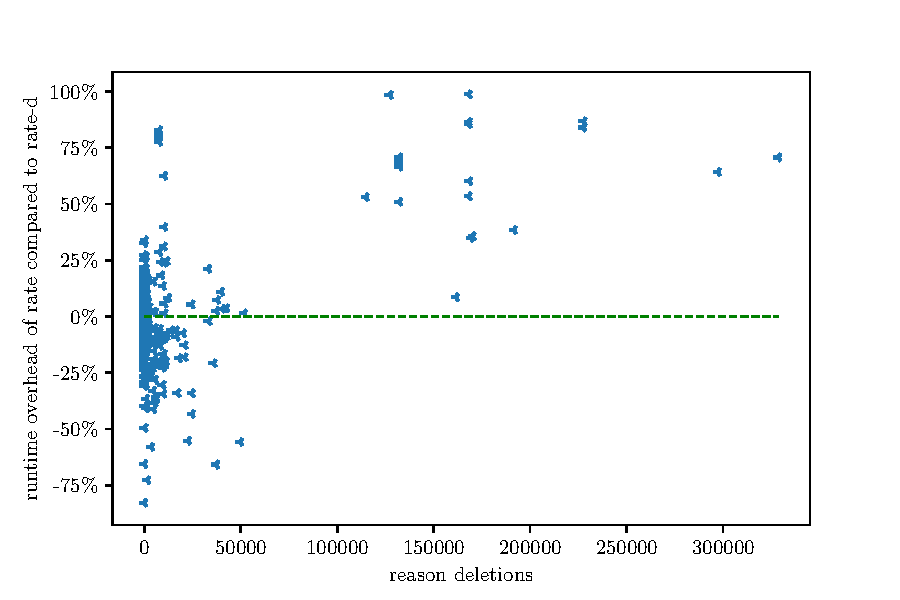
\includegraphics{p/correlation-reason-deletions-time-delta-percent.pdf}
\caption{Juxtaposition of the number of reason deletions and the
relative runtime overhead of checking specified DRAT over operational
DRAT.\label{fig:correlation-reason-deletions-time-delta-percent}}
\end{figure}

\begin{figure}
\centering
\includegraphics{p/correlation-reason-deletions-space-delta-percent.pdf}
\caption{Juxtaposition of the number of reason deletions and the
relative overhead in terms of memory usage of checking specified DRAT
over operational
DRAT.\label{fig:correlation-reason-deletions-space-delta-percent}}
\end{figure}

\hypertarget{overhead-of-reason-deletions}{%
\section{5.2 Overhead of Reason
Deletions}\label{overhead-of-reason-deletions}}

Figure \ref{fig:correlation-reason-deletions-time-delta-percent}
suggests that a large number of reason deletions brings about some
runtime overhead in \texttt{rate} when checking specified DRAT as
opposed to operational DRAT. Same holds for memory usage as can be seen
in Figure \ref{fig:correlation-reason-deletions-space-delta-percent}.
Currently, \texttt{rate} incurs these extra costs also for proofs that
contain no unique reason deletions.

\hypertarget{conclusion}{%
\chapter{6. Conclusion}\label{conclusion}}

In
\protect\hyperlink{drat-proofs-without-deletions-of-unique-reason-clauses}{Section
3} we have explained why operational DRAT is required to verify
\texttt{DRUPMiniSat}-based solvers' proofs. We have proposed patches for
these solvers to create proofs that are correct under either flavor and
do not require ignoring unit deletions.

Specified DRAT is necessary to verify solvers' inprocessing steps that
employ deletions of unique reason clauses
{[}\protect\hyperlink{ref-rebola2018two}{4}{]}. We implement an
efficient checker, \texttt{rate}, that supports both specified and
operational DRAT. Furthermore, specified DRAT features the advantage
that the accumulated formula is easy to compute without performing unit
propagation. This enables us to produce SICK certificates which are
small, efficiently checkable witnesses of a proof's incorrectness. They
report which proof step failed, which can be used to detect bugs in
checkers and pinpoint bugs in solvers. We provide a tool,
\texttt{sick-check} to check SICK witnesses.

Our initial research question was whether specified DRAT can be checked
as efficiently as operational DRAT. Based on our benchmarks we provided
evidence that the cost for specified DRAT is, on average, the same but
an excessive number of reason deletions can make it significantly more
costly.

\hypertarget{future-work}{%
\chapter{7. Future Work}\label{future-work}}

If a checker for specified DRAT were to be adopted, it might be
beneficial to implement a way to perform deletions of non-unique reasons
more efficiently than \texttt{rate} does. These deletions do not alter
the shared UP-model, but \texttt{rate} does not know this. An
optimization could consist of an efficiently computable criterion to
determine if some reason clause is unique. A simple criterion is as
follows: if a reason clause for some literal \(l\) is deleted, check if
unit clause \(l\) is in the formula. If it is, then the deleted reason
is not unique and the shared UP-model will definitely not change. This
criterion might be sufficient for the proofs produced by the second
variant of the patches from
\protect\hyperlink{drat-proofs-without-deletions-of-unique-reason-clauses}{section
3}.

State-of-the-art DRAT checkers are heavily optimized for speed but they
keep the entire input proof and the resulting LRAT proof in memory. If
the available memory is at premium, some changes could be made to do
backwards checking in a streaming manner. Additionally, the LRAT proof
output could be streamed as well, with some postprocessing to fix the
clause IDs.

It might be possible to forego DRAT completely and directly generate
LRAT in a solver which is done by \texttt{varisat}. This removes the
need for a complex checker at the cost of a larger proof artifact.

\if0 DRAT: 414101681719 LRAT: 294413262360 (core only) \fi

\hypertarget{references}{%
\chapter*{References}\label{references}}
\addcontentsline{toc}{chapter}{References}

\hypertarget{refs}{}
\leavevmode\hypertarget{ref-BrummayerBiere-SMT09}{}%
{[}1{]} R. Brummayer and A. Biere, ``Fuzzing and delta-debugging smt
solvers,'' \emph{ACM International Conference Proceeding Series}, pp.
1--5, Jan. 2009.

\leavevmode\hypertarget{ref-BrummayerLonsingBiere-SAT10}{}%
{[}2{]} R. Brummayer, F. Lonsing, and A. Biere, ``Automated testing and
debugging of sat and qbf solvers,'' 2010, vol. 6175, pp. 44--57.

\leavevmode\hypertarget{ref-Heule_2014}{}%
{[}3{]} M. J. H. Heule, W. A. Hunt, and N. Wetzler, ``Bridging the gap
between easy generation and efficient verification of unsatisfiability
proofs,'' \emph{Software Testing, Verification and Reliability}, vol.
24, no. 8, pp. 593--607, Sep. 2014.

\leavevmode\hypertarget{ref-rebola2018two}{}%
{[}4{]} A. Rebola-Pardo and A. Biere, ``Two flavors of drat,''
\emph{Pragmatics of SAT}, vol. 2018, 2018.

\leavevmode\hypertarget{ref-schur-5}{}%
{[}5{]} M. J. H. Heule, ``Schur number five,'' Nov. 2017.

\leavevmode\hypertarget{ref-RebolaCruz2018}{}%
{[}6{]} A. Rebola-Pardo and L. Cruz-Filipe, ``Complete and efficient
drat proof checking,'' 2018.

\leavevmode\hypertarget{ref-Moskewicz:2001:CEE:378239.379017}{}%
{[}7{]} M. W. Moskewicz, C. F. Madigan, Y. Zhao, L. Zhang, and S. Malik,
``Chaff: Engineering an efficient sat solver,'' in \emph{Proceedings of
the 38th annual design automation conference}, 2001, pp. 530--535.

\leavevmode\hypertarget{ref-cdcl}{}%
{[}8{]} J. Marques-Silva, I. Lynce, and S. Malik, ``Conflict-driven
clause learning sat solvers,'' in \emph{Handbook of satisfiability}, 1st
ed., Netherlands: IOS Press, 2009, pp. 131--153.

\leavevmode\hypertarget{ref-Heule_2017}{}%
{[}9{]} M. J. H. Heule, B. Kiesl, and A. Biere, ``Short proofs without
new variables,'' \emph{Lecture Notes in Computer Science}, pp. 130--147,
2017.

\leavevmode\hypertarget{ref-rup}{}%
{[}10{]} A. Van Gelder, ``Verifying rup proofs of propositional
unsatisfiability.'' 2008.

\leavevmode\hypertarget{ref-inprocessingrules}{}%
{[}11{]} M. Järvisalo, M. Heule, and A. Biere, ``Inprocessing rules,''
2012, vol. 7364.

\leavevmode\hypertarget{ref-rat}{}%
{[}12{]} M. J. H. Heule, W. A. Hunt, and N. Wetzler, ``Verifying
refutations with extended resolution,'' in \emph{Automated deduction --
cade-24}, 2013, pp. 345--359.

\leavevmode\hypertarget{ref-Wetzler_2014}{}%
{[}13{]} N. Wetzler, M. J. H. Heule, and W. A. Hunt, ``DRAT-trim:
Efficient checking and trimming using expressive clausal proofs,''
\emph{Theory and Applications of Satisfiability Testing -- SAT 2014},
pp. 422--429, 2014.

\leavevmode\hypertarget{ref-philipp_rebola_unsatproofs}{}%
{[}14{]} T. Philipp and A. Rebola-Pardo, ``Towards a semantics of
unsatisfiability proofs with inprocessing.''

\leavevmode\hypertarget{ref-cruz2017efficient}{}%
{[}15{]} L. Cruz-Filipe, M. J. Heule, W. A. Hunt, M. Kaufmann, and P.
Schneider-Kamp, ``Efficient certified rat verification,'' in
\emph{International conference on automated deduction}, 2017, pp.
220--236.

\leavevmode\hypertarget{ref-Heule_2013}{}%
{[}16{]} M. J. H. Heule, W. A. Hunt, and N. Wetzler, ``Trimming while
checking clausal proofs,'' \emph{2013 Formal Methods in Computer-Aided
Design}, Oct. 2013.

\leavevmode\hypertarget{ref-lammich2017grat}{}%
{[}17{]} P. Lammich, ``The grat tool chain,'' in \emph{International
conference on theory and applications of satisfiability testing}, 2017,
pp. 457--463.

\leavevmode\hypertarget{ref-lammich2017efficient}{}%
{[}18{]} P. Lammich, ``Efficient verified (un) sat certificate
checking,'' in \emph{International conference on automated deduction},
2017, pp. 237--254.

\leavevmode\hypertarget{ref-Tange2018}{}%
{[}19{]} O. Tange, \emph{GNU parallel 2018}. Ole Tange, 2018.

\end{document}
